\providecommand\ExamFontPath{../../../字体/}
\documentclass[fontset=exam]{exam-zh}
\usepackage{longtable,booktabs,array,calc,multirow,fvextra}
\usepackage[normalem]{ulem}
\providecommand{\hl}[1]{#1}
\providecommand{\ul}[1]{\uline{#1}}
\DefineVerbatimEnvironment{verbatim}{Verbatim}{breaklines=true,fontsize=\small}
\providecommand{\tightlist}{\setlength{\itemsep}{0pt}\setlength{\parskip}{0pt}}
\newcommand{\pandocbounded}[1]{#1}
\setlength{\emergencystretch}{3em}
\setlength{\tabcolsep}{2pt}
\examsetup{page/size=a4paper}
\title{厦门大学 2009 级期末试卷}
\subject[4em]{力学}
\begin{document}
\maketitle
\fancyfoot[C]{第 \thepage 页（共 \pageref*{LastPage} 页）}
\pdfbookmark[1]{一． 判断题（每小题2分，共20分。正确的在相应序号后打“√”，错误的打“×”。要求将答案写在答题纸上）}{section1}

一． 判断题（每小题 2 分，共 20 分。正确的在相应序号后打``√''，错误的打``×''。要求将答案写在答题纸上）

\begin{enumerate}
\def\labelenumi{\arabic{enumi}.}
\item
  作用在刚体上的外力的矢量和为零时，刚体的运动状态一定不变
\item
  当物体纯滚动时，作用在物体上的静摩擦力总是与物体质心的运动方向相反
\item
  物体的质量越大，转动惯量也越大
\item
  两同方向、同频率简谐振动合成后仍然为简谐振动
\item
  驻波不是平面简谐波
\item
  波速与质元的振动速度成正比
\item
  一波源产生的平面简谐横波一段时间后将振动传播至某质点，该质点初始振动方向取决于它离波源的位置
\item
  定常流动时的流线与流迹相重合
\item
  真空中的光速对任何惯性参考系都相同
\end{enumerate}

10.高速运动的电子其质量随其速率增大而增大

\pdfbookmark[1]{二．(16分) 一长度为l，质量为m的均质细杆从静止开始由竖直位置自然倒下。已知桌面光滑。求：}{section4}

二．(16 分) 一长度为\(l\)，质量为\(m\)的均质细杆从静止开始由竖直位置自然倒下。已知桌面光滑。求：\par\medskip{\centering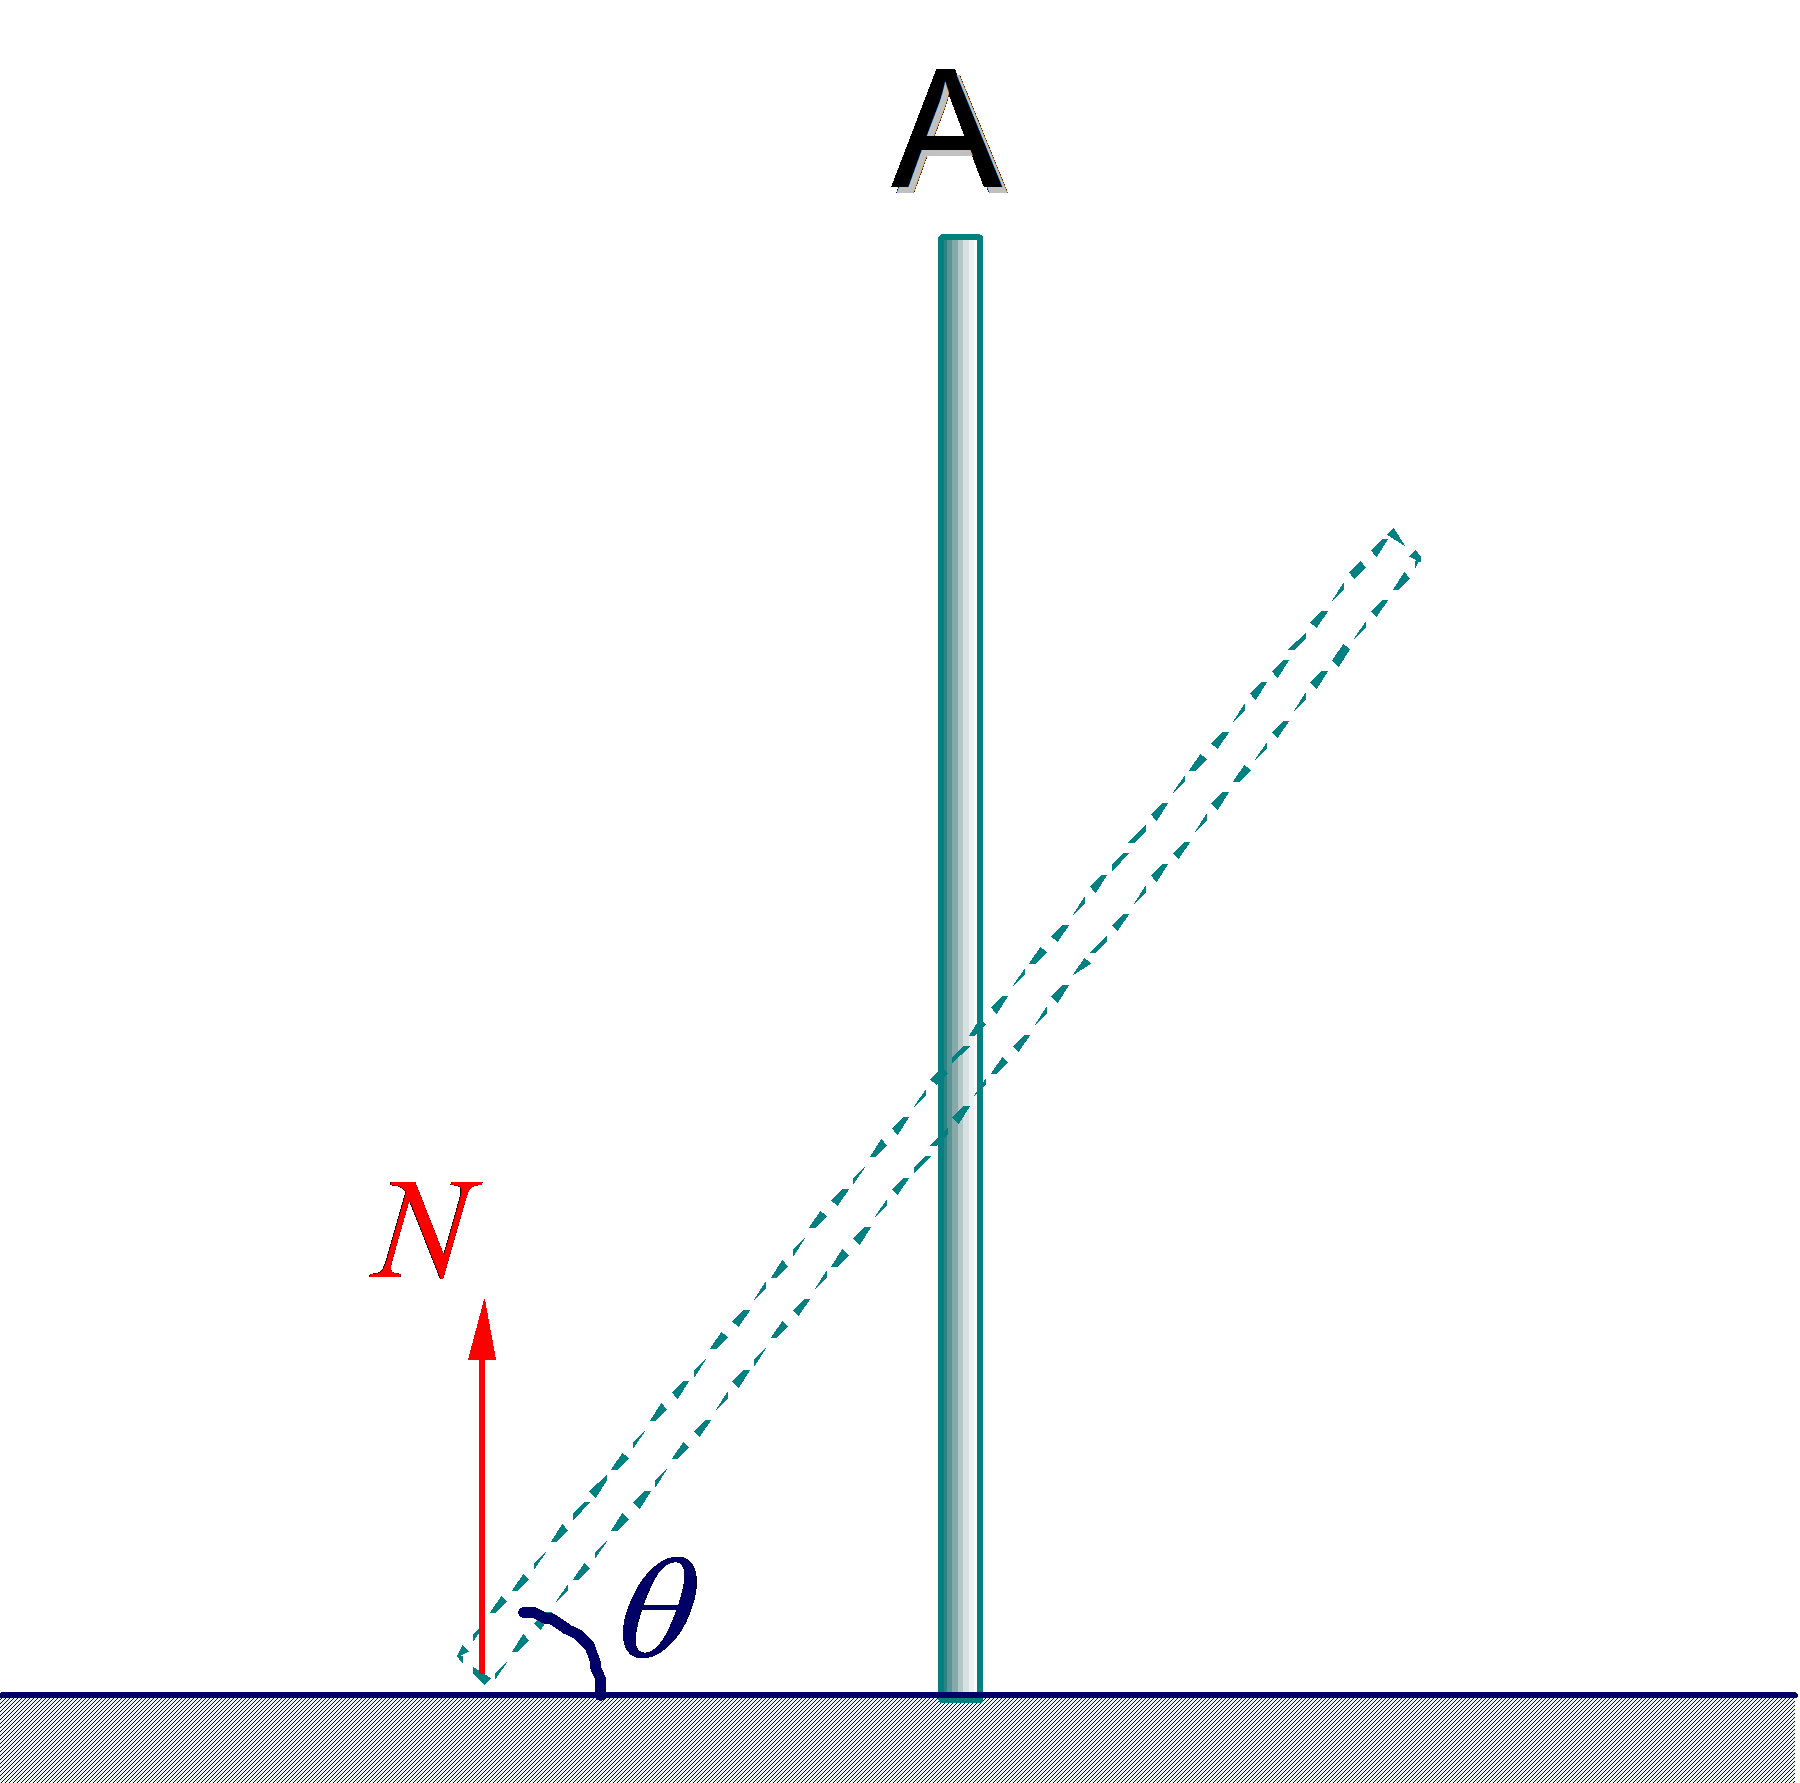
\includegraphics[width=5cm,height=4cm,keepaspectratio]{figures/image2.png}\par}\medskip

（1）若以最初杆与地面的接触点为坐标原点建立直角坐标系，求杆的端点 A 的轨道方程

（2）杆与水平地面夹角为\(\theta\)时，杆质心的速度和杆的角速度；

（3）细杆即将倒地瞬间地面对杆的支撑力\emph{N}。

\pdfbookmark[1]{三．(16分) 如图所示，质量为m, 半径为R的均质薄圆盘，其初角速度为omega_0。若空气对圆盘表面单位面积的磨擦力}{section8}

三．(16 分) 如图所示，质量为 m, 半径为 R 的均质薄圆盘，其初角速度为\(\omega_{0}\)。若空气对圆盘表面单位面积的磨擦力\(F_{f}\)正比于该处的线速度\(v\)（即\(F_{f} = kv\)，\(k\)为常数）, 且不计轴承处磨擦，试求：\par\medskip{\centering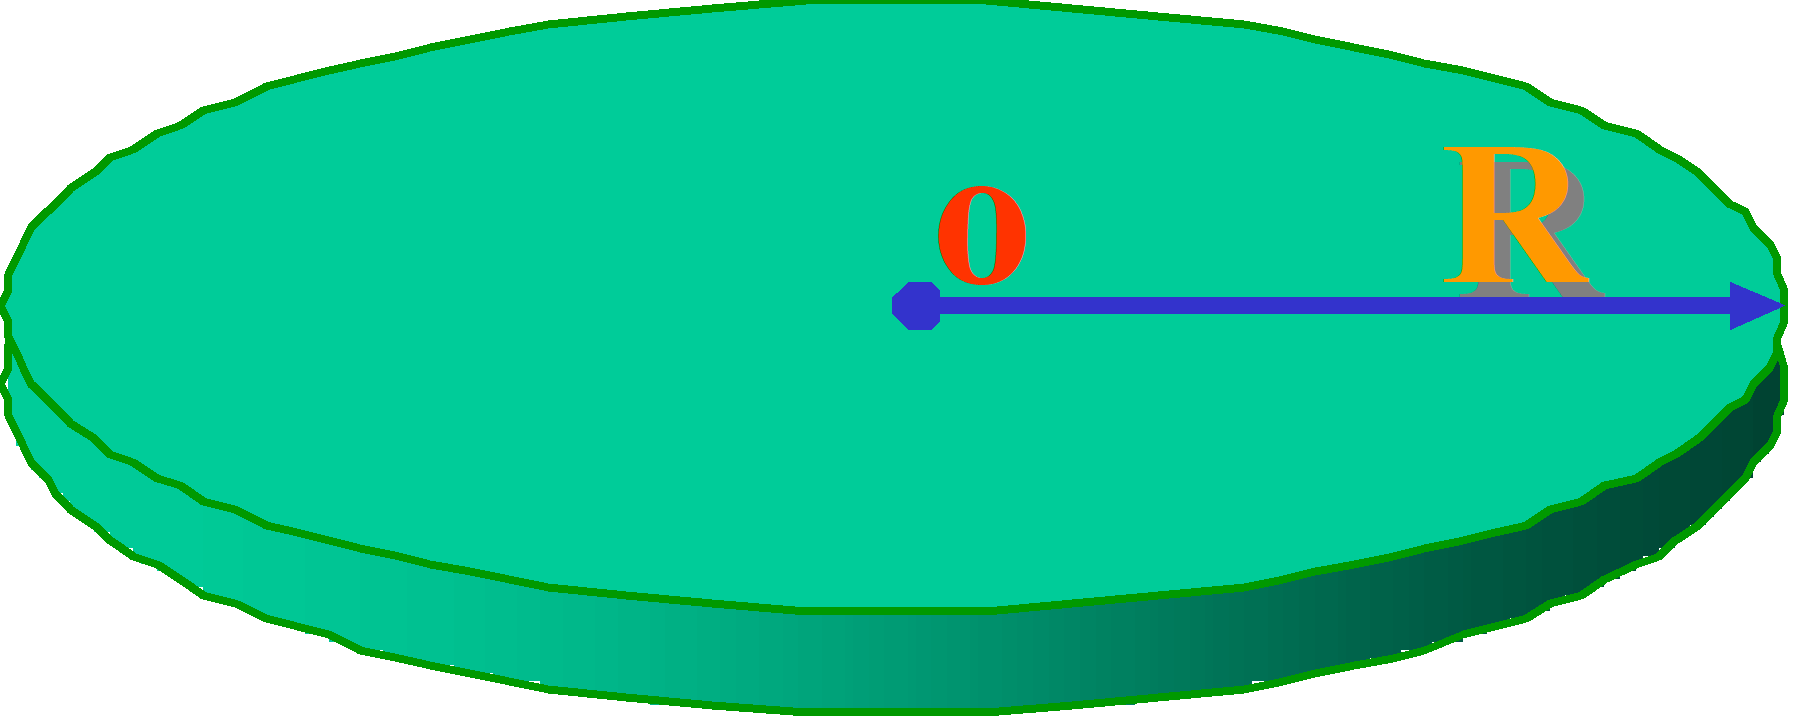
\includegraphics[width=5cm,height=4cm,keepaspectratio]{figures/image6.png}\par}\medskip

（1）当圆盘转动角速度为\(\omega\)时所受空气阻力矩

（2）圆盘停止转动前所转过的圈数

\pdfbookmark[1]{四．(16分) 如图所示，已知弹簧的劲度系数为k，物体的质量为m，滑轮的半径为R，质量为M。开始时托住物体m，使得系统保}{section11}

四．(16 分) 如图所示，已知弹簧的劲度系数为 k，物体的质量为 m，滑轮的半径为 R，质量为 M。开始时托住物体 m，使得系统保持静止，绳子刚好拉直而弹簧无形变，t=0 时放开 m。设绳子与滑轮间无相对滑动，滑轮可视为均质圆盘。\par\medskip{\centering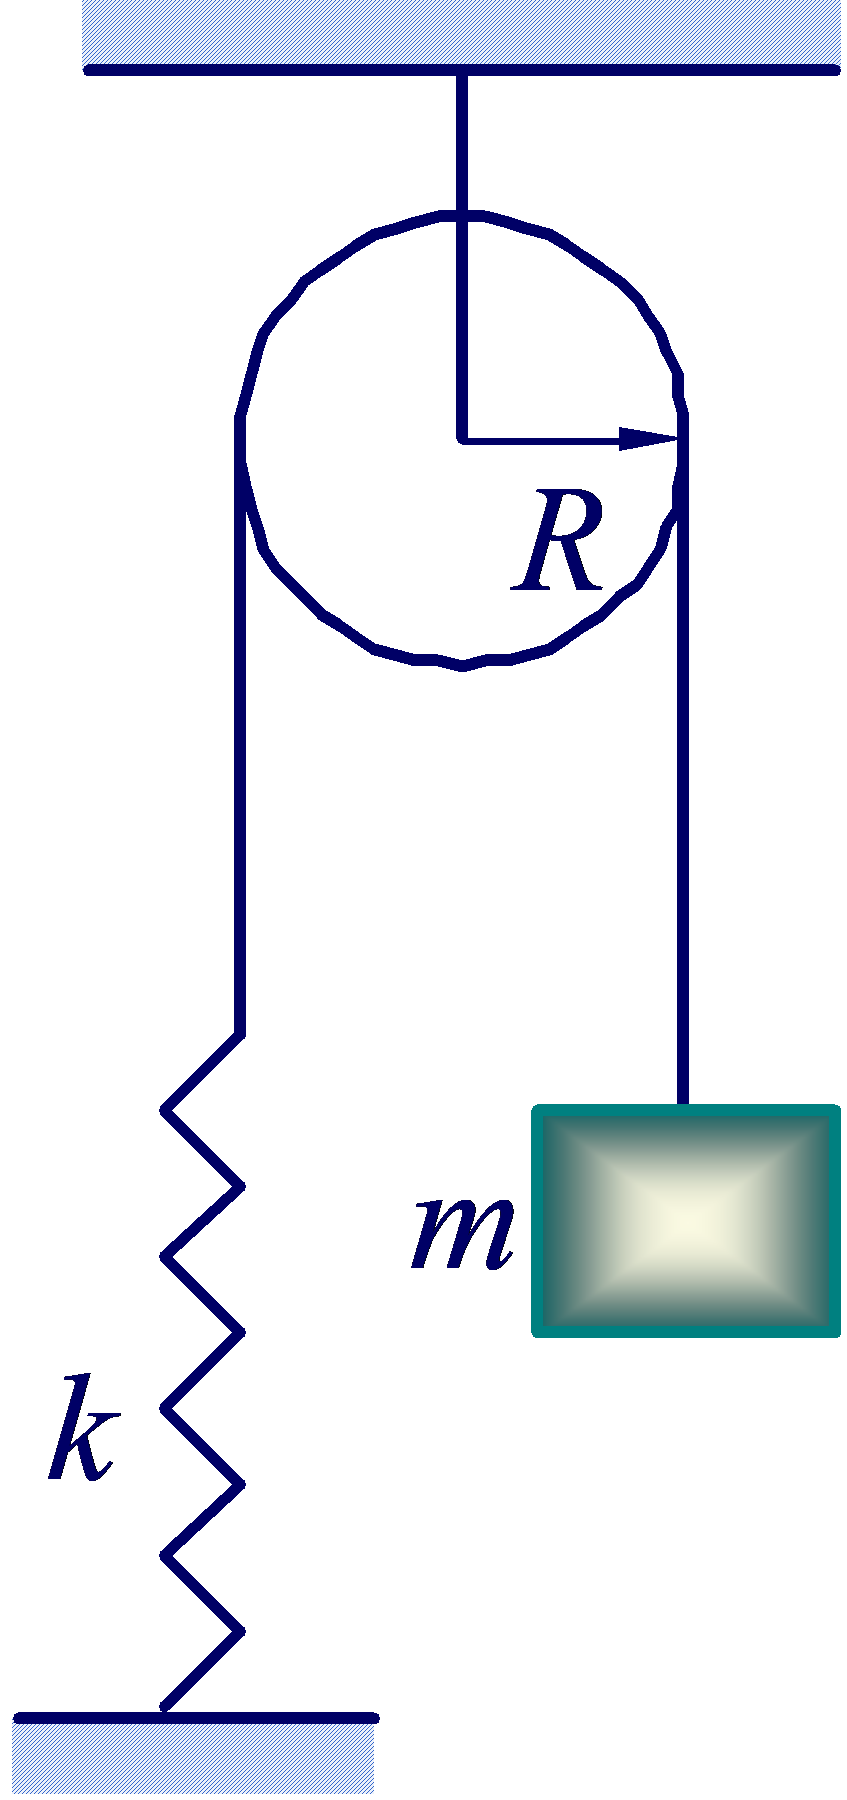
\includegraphics[width=5cm,height=4cm,keepaspectratio]{figures/image13.png}\par}\medskip

(1)放开后 m 是否作简谐振动？若是，试求出振动周期 T；

(2)写出 m 的振动表达式。

\pdfbookmark[1]{五．(16分) 原点处产生的一平面简谐波以波速u=4m/s沿x轴正方向传播，已知t=0时的波形图如图所示。若该波在x=L}{section14}

五．(16 分) 原点处产生的一平面简谐波以波速 u=4m/s 沿 x 轴正方向传播，已知 t=0 时的波形图如图所示。若该波在 x=L 处发生界面反射，且反射时无半波损失。试求:\par\medskip{\centering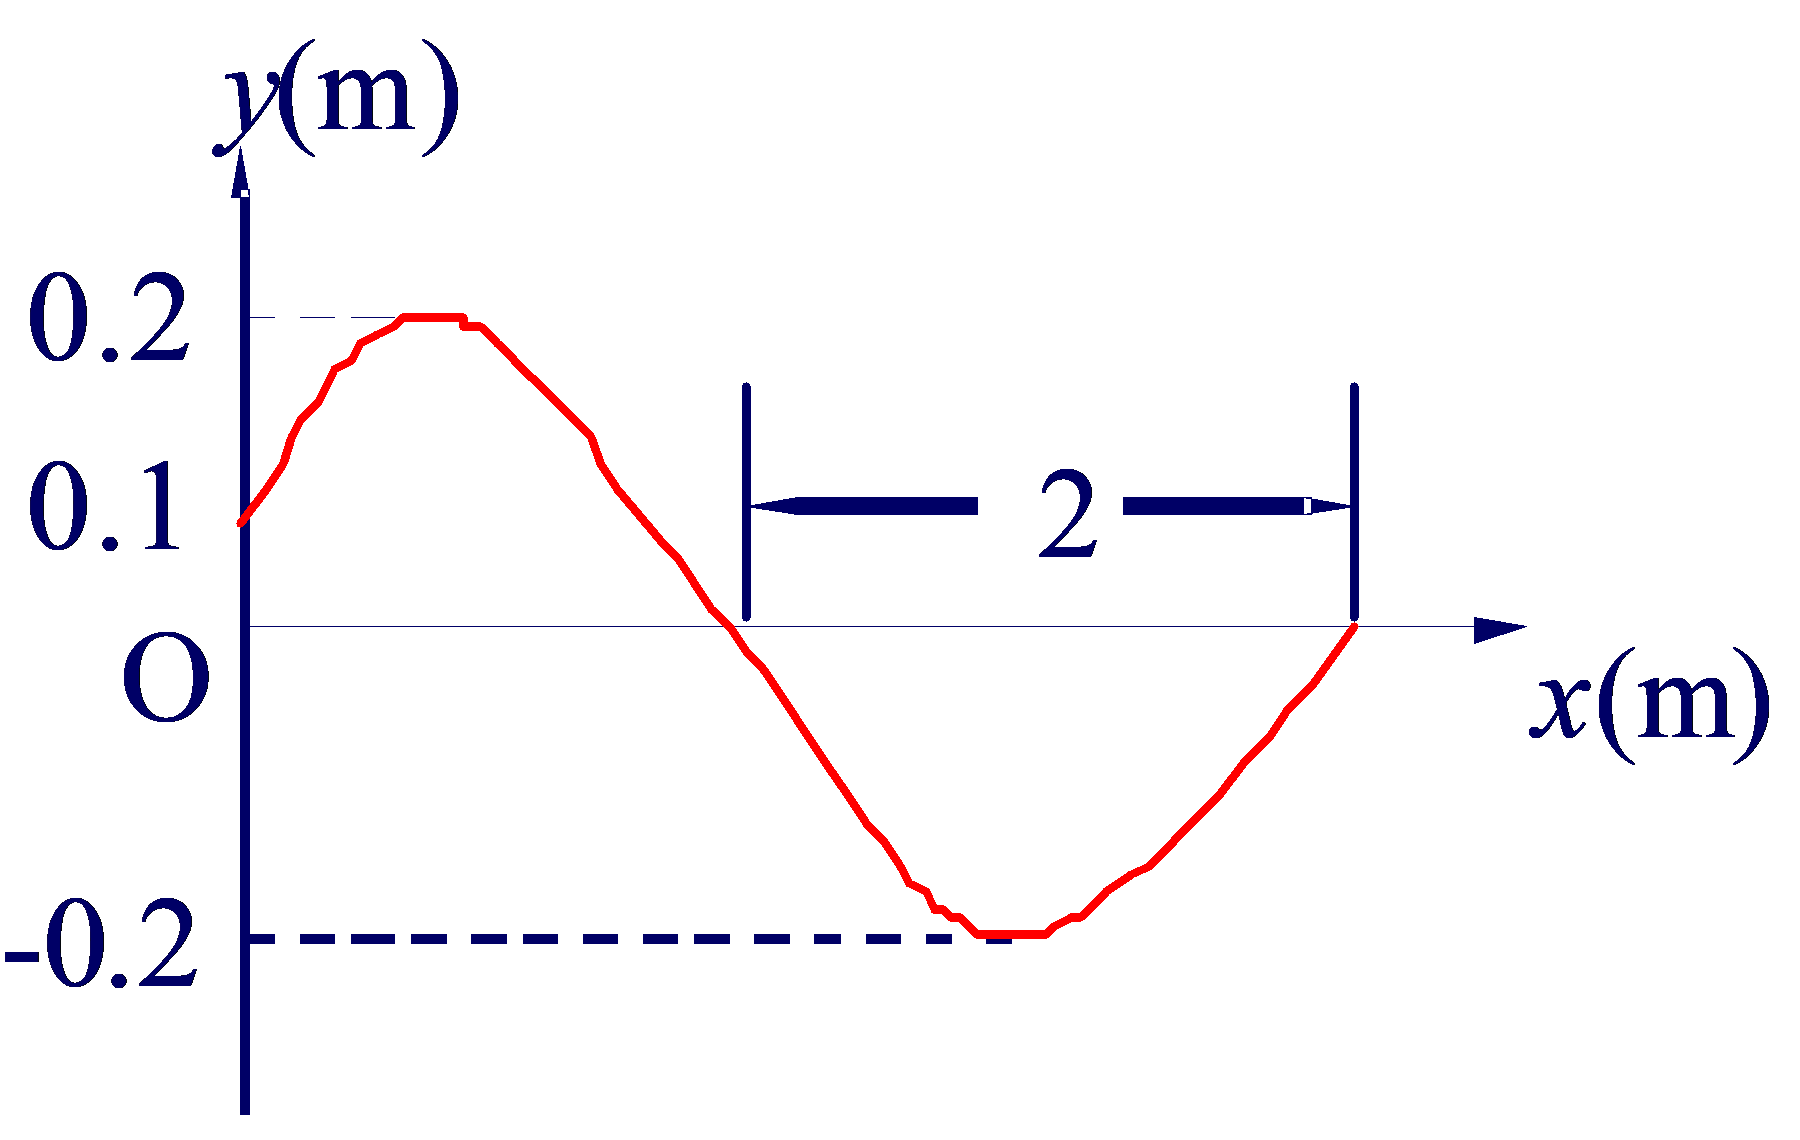
\includegraphics[width=5cm,height=4cm,keepaspectratio]{figures/image14.png}\par}\medskip

(1)原点处的振动方程

（2）该平面简谐波的波函数

(3)反射波的波函数（不考虑振幅衰减）

(4)若 L=10m 且波在反射时发生半波损失，请直接写出原点与反射点之间所有波节的位置坐标。

\pdfbookmark[1]{六. (16分) 一飞船A以0.8c的速度平行于地面飞行。宇航员测得此飞船的长度为100米。问：}{section19}

六. (16 分) 一飞船 A 以 0.8c 的速度平行于地面飞行。宇航员测得此飞船的长度为 100 米。问：

（1）地面上的观测者测得的飞船 A 的长度为多少？

（2）地面上的观测者为测量 A 飞船长度，需有两位观测者携带两只同步的钟同时地测量 A 飞船两端。宇航员测得地面上的观测者相距有多远？

（3）若有另一飞船 B 相对地面以 0.8c 的速度沿相反方向飞行，问 A 飞船上的观测者所测得的 B 飞船的速度大小。

\end{document}
